% !TeX root = ../document.tex
\documentclass[../document.tex]{subfiles}
\lstset{inputpath=sections}
\begin{document}

	\subsection{Overview (What is Statistical Learning)}

	\paragraph{General}
	We assume that there (in a dataset) is a fixed but unknown relationship between the input variables (vector X) and the output variables (vector Y).
	\begin{equation} \label{eq:1}
	X = (X_{1},X_{2},...,X_{p})
	\end{equation}
	\begin{equation} \label{eq:2}
	Y=f(X)+\epsilon
	\end{equation}
	Where \(\epsilon\) is the random term and is independent of X.
	We would like to predict the outcome , given we know the input variable. But normally we don't know the function. Therefore we would like to learn the function from a given dataset, which is called statistical learning.\\
	\begin{equation} \label{eq:3}
	\hat{Y} = \hat{f}(X)
	\end{equation}
	Only an estimate of the function f therefore it's \(\hat{f}\). We are only concerned with the quality of the estimated \(\hat{Y}\)
	As in \ref{eq:1} mentioned, the X value is often a vector. And as in \ref{eq:2} mentioned, we can measure the prediction accuracy.\\

	\paragraph{Errors}
	There are 2 types of errors (irreducible and reducible)\\
	The irreducible error is the \(\epsilon\) in \ref{eq:2}, whereas the reducible error is the difference from our estimated function to the real function.
	\begin{equation}
	\begin{split}
	E(Y-\hat{Y})^2 &= E[f(X)+\epsilon-\hat{f}(X)]^2 \\
	&= [f(X)-\hat{f}(X)]^2+Var(\epsilon)
	\end{split}
	\end{equation}
	The first part (before the plus) is the reducible error, or how well we estimated the function. The second part is the irreducible error which is given. In total we get the prediction accuracy, which is measured in the mean of the squared error (MSE).

	\paragraph{Inference}
	In contrast to the prediction, with inference we would like to understand how the input variables (predictors) influence the output variables (response). We need models which can be easily understood, because interference is a much harder problem than prediction.

	\paragraph{parametric}
	A parametric approach for estimating f uses assumptions about the form of f, where only some missing parameters need to be learned.
	\begin{equation}
	f(X) = \beta_{0}+\beta_{1}X_{1}+\beta_{2}X_{2}+...+\beta_{n}X_{n}
	\end{equation}
	The precision of the function depends on the numbers of parameters, but maybe we have to much parameters and overfit the training data.

	\paragraph{non-parametric}
	There is no assumption about the form of the function and the idea is to create a surface, which approximates the given datapoints, without being to rough or to wiggly. They need in general more data to predict better.

	\paragraph{supervised vs. unsupervised}
	Supervised means that we know each output Y of a given X. The opposite is unsupervised learning, where we don't know the right Y and the model has to find some structure in the data.

	\paragraph{regression vs. classification}
	Variables can be quantitative (numerical) where we have a regression problem, or qualitative (categorical) where we have a classification problem (where Y is numerical or categorical).


	\subsection{Assessing Model Accuracy}

	\paragraph{Quality of fit (fitness)}
	So that we can select an appropriate learning method, we need a function to evaluate the performance of the method. One popular measure is the mean squared error (MSE).
	\begin{equation}
	MSE = \frac{1}{n}\sum_{i=1}^{n} (y_{i}-\hat{f}(x_{i}))^2
	\end{equation}
	\begin{equation}
	Ave(y_{0}-\hat{f}(x_{0}))^2
	\end{equation}
	We need to make a performance analysis with a test dataset, which the function has never seen before.\\
	Unfortunately we can't just select a low MSE, because this would lead to overfit, worsening the model's ability to generalize to new data.\\
	\begin{center}
		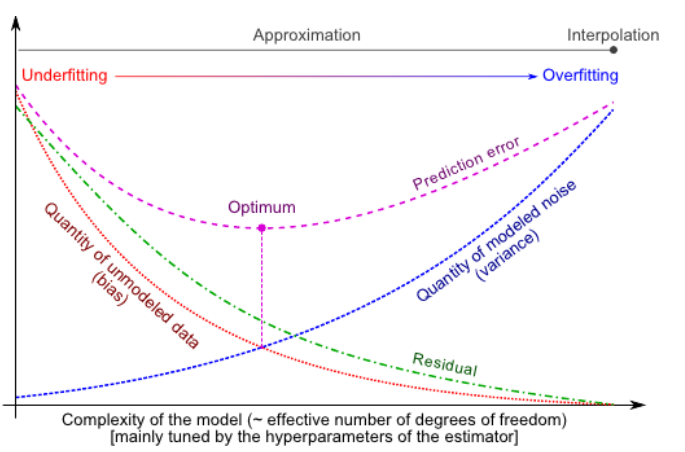
\includegraphics[width=.7\textwidth]{pictures/variance_bias_tradeoff.png}
	\end{center}


	\paragraph{bias vs. variance}
	The expected test MSE can be built with the sum of a variance term, a bias term and the irreducible error.
	\begin{equation}
	E(y_{0}-\hat{f}(x_{0}))^2 = Var(\hat{f}(x_{0})) + [Bias(\hat{f}(x_{0}))]^2 + Var(\epsilon)
	\end{equation}
	This estimated MSE is a repeated f over a large number of training sets. So to minimize the expected MSE, we need to find a method with low variance and low bias.\\
	\subparagraph{variance}
	New points (other test data) should have no influence (low variance) - low flexibility
	\subparagraph{bias}
	Bias is the error of the method. So the distance of the real points to the function. (low bias) - high flexibility

	\paragraph{classification}
	To measure the fitness of a classification method, we must count each wrong classification of a data point.
	\begin{equation}
	\frac{1}{n}\sum_{i=1}^{n}I(y_{i} \neq \hat{y}_{i})
	\end{equation}
	\begin{equation}
	Ave(I(y_{0} \neq \hat{y}_{0}))
	\end{equation}
	A good classifier is a classifier with a low test error rate.

	\paragraph{bayes classifier}
	The bayes classifier picks for each observation the most likely class to minimize the average of the test error. Given an input variable (predictor) X, pick the class (response) Y, which is te most probable one.
	\begin{equation}
	Pr(Y=j|X=x_{0})
	\end{equation}
	When we have a set with 2 different classes as output, the bayes classifier has an averaged error rate of 0.1304, which is greater than 0, since the classes overlap in the true population. The bayes error rate is analogous to the irreducible error.
	\begin{equation}
	1 - E(maxPr(Y=j|X)) = 0.1304
	\end{equation}

	\paragraph{K-nearest neighbors}
	The bayes classifier requires the knowledge of the conditional distribution of Y given X. This is never known and we try to imitate the best possible value. One method is K-nearest neighbors. Given a test point \(x_{0}\), the method finds the K nearest neighbors \(N_{0}\) an then estimates the class probabilities as the fraction of the K neighbors, which belong to a particular class. Then the highest estimated class probability is selected.
	\begin{equation}
	Pr(Y=j|X=x_{0})=\frac{1}{K}\sum_{i \in N_{0}} I(y_{i}=j)
	\end{equation}
	If the K is too small, then the KNN classifier follows the noise of the training data very closely and hence the variance is large. If the K is too large, then the KNN classifier isn't very accurate and hence the bias very large.



\end{document}
